\documentclass{beamer}
\usepackage{tikz}
\usepackage{multicol}
\usepackage{pgfplots}
\usepackage{amsmath}
\usepackage{xcolor}
\usepackage{bm}
\usepackage{algorithm}
\usepackage{algpseudocode}
\usepackage{amsthm, amssymb, amsmath}
\usepackage{stmaryrd}
\usepackage{changepage}
\usepackage{parskip}
\usepackage{hyperref}
\usepackage{wasysym}
\usepackage{subcaption}
\usepackage{comment}
\pgfplotsset{compat=1.18}
\title{CSE380 Group Presentation:\\
Poisson Equation Solver in 2D Domain}
\author{Group 5: Alwin Anto, Judy Hao, Shan Jiang, Bowen Shi}
\date{December 2024}
\setbeamertemplate{footline}{}

\newcommand{\abs}[1]{\left|#1\right|}
\newcommand{\sabs}[1]{|#1|}
\newcommand{\bs}[1]{\boldsymbol{#1}}
\newcommand{\pp}[2]{\frac{\partial {#1}}{\partial {#2}}}
\newcommand{\db}[1]{\llbracket{#1}\rrbracket}
\newcommand{\ora}[1]{\overrightarrow{#1}}
\newcommand\bigzero{\makebox(0,0){\text{\huge0}}}

\begin{document}
\frame{\titlepage}
\begin{frame}[t]{Table of Contents}
    \small % Or \footnotesize
    \tableofcontents[hideallsubsections]
\end{frame}

\section{Introduction}
\begin{frame}{Introduction}
\textcolor{blue}{Objective}: Solve the Poisson equation on a rectangular domain using the finite element method (FEM), validate it with the analytical solution, and evaluate the convergence behavior.\vspace{0.5cm}

\textcolor{blue}{Tool/Techniques}: CMake, Docker, GDB, TPL (Eigen, HDF5), Input parsing, Convergence Analysis, gprof, valgrind
\end{frame}

\section{Problem Formulation}
\begin{frame}{Problem Formulation}
Consider the Poisson equation on the rectangular domain $\Omega=(0,1) \times (0,1)$,
$$
-\Delta u = f, \quad (x, y) \in \Omega.
$$
with the boundary conditions
\begin{align*}
    u = g_1,\quad& (x, y) \in \partial \Omega_0 \\
\frac{\partial u}{\partial \boldsymbol{n}} = g_2, \quad& (x, y) \in \partial \Omega_1
\end{align*}
where $\partial \Omega_0 = \{0\} \times [0,1]$, and $\partial \Omega_1 = \partial \Omega - \partial \Omega_0$.
\end{frame}

\section{Solution Approach}
\subsection{Principle}
\begin{frame}{Principle}
Set $f = 1 + n \cos(\pi y), \quad g_1(y)=0,\quad g_2(x, y)=0.$
\\Take the test function $v \in \mathbb{V}:=\left\{v \in \mathbb{H}^{1}(\Omega) \mid v|_{\partial \Omega_{0}}=0\right\}$.
\\ $$
-\int_{\Omega} \Delta u \cdot v=\int_{\Omega} \nabla u \cdot \nabla v-\int_{\partial \Omega} \frac{\partial u}{\partial \boldsymbol{n}} \cdot v=\int_{\Omega} \nabla u \cdot \nabla v
$$
\\The variational form is: \begin{equation*}
\int_{\Omega} \nabla u \cdot \nabla v=\int_{\Omega} f v
\end{equation*}
\pause
Also, propose functional minimization problem: 
$$
J(u)=\min_{v \in \mathbb{V}} J(v),\quad J(v)=\frac{1}{2} \int_{\Omega}|\nabla v|^{2}-\int_{\Omega} f v
$$
\end{frame}

\subsection{Finite Element Method and Algorithm}
\begin{frame}{Finite Element Method}
Notation: $h$ denote the element diameter in the mesh, $N$ the number of nodes, and $M$ the number of elements
    \begin{figure}[h]
    \centering
    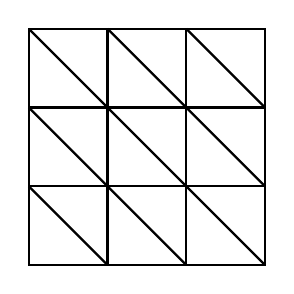
\begin{tikzpicture}[scale=3]
        % Draw the outer square
        \draw[thick] (0, 0) rectangle (1, 1);

        % Draw the grid for the 9 sub-squares
        \draw[thick] (1/3, 0) -- (1/3, 1);
        \draw[thick] (2/3, 0) -- (2/3, 1);
        \draw[thick] (0, 1/3) -- (1, 1/3);
        \draw[thick] (0, 2/3) -- (1, 2/3);

        % Draw the diagonals for each sub-square from bottom right to upper left
        \foreach \i in {0, 1, 2} {
            \foreach \j in {0, 1, 2} {
                \draw[thick] ({(\i+1)/3}, {\j/3}) -- ({\i/3}, {(\j+1)/3}); % Draw diagonal from bottom right to upper left
            }
        }
    \end{tikzpicture}
    \caption{A unit square divided into 9 sub-squares, each subdivided into two triangles.}
    \label{fig:mesh}
\end{figure}
\end{frame}
\begin{frame}{Finite Element Method Cont.}
$P_1$ Lagrange finite element space: $$
\mathbb{V}_{h}=\left\{u \in C(\bar{\Omega}): \left.u\right|_{T_{i}} \in \mathbb{P}_{1}\left(T_{i}\right), \forall T_{i} \in \mathcal{T}_{h}(\Omega)\right\}
$$
\pause 
Finite element trial function space and test function space:
$$
\mathbb{V}_{h}\left(0 ; \Omega_{0}\right)=\left\{u \in \mathbb{V}_{h}: u\left(A_{i}\right)=0, \forall A_{i} \in \partial \Omega_{0}\right\}
$$
\pause
Problem:
Find \( u_h \in \mathbb{V}_h(0; \Omega_0) \) such that:
\[
a(u_h, v_h) = F(v_h), \quad \forall v_h \in \mathbb{V}_h(0; \Omega_0)
\]
$$\text{where \quad}
a(u, v)=\int_{\Omega} \nabla u \cdot \nabla v, \quad F(v)=\int_{\Omega} f v
$$    
\end{frame}

\begin{frame}{Finite Element Method Cont.}
Let $\varphi_{i} \in \mathbb{V}_{h}$ satisfy
$$
\varphi_{i}\left(A_{j}\right)=\delta_{i j}, \quad i=1,2, \dots, N
$$

$\left\{\varphi_{i}\right\}_{i=1}^{N}$ forms a basis for $\mathbb{V}_{h}$, $\left\{\varphi_{i}\right\}_{A_{i} \notin \partial \Omega_{0}}$ forms basis for $\mathbb{V}_{h}\left(0 ; \Omega_{0}\right)$
\pause
Let
$$
u_{h}=\sum_{j=1}^{N_{h}} u_{j} \varphi_{j}, \quad v_{h}=\sum_{i=1}^{N_{h}} v_{i} \varphi_{i}\text{ , where }N_{h}=\frac{1}{h^{2}}+\frac{1}{h}
$$
The discrete problem is equivalent to:
$$
\sum_{j=1}^{N_{h}} a\left(\varphi_{j}, \varphi_{i}\right) u_{j}=F\left(\varphi_{i}\right), \quad i=1,2, \dots, N_{h}
$$
\end{frame}

\begin{frame}{Algorithm}

\begin{equation*}
\boldsymbol{K} \boldsymbol{u}_{h} = \boldsymbol{f} \label{eq:stiff}
\end{equation*}

\begin{algorithm}[H]
\caption{Algorithm for forming the stiffness matrix and load vector}
\begin{algorithmic}[1] % The `[1]` adds line numbers
    \State \textbf{Input:} $\boldsymbol{K} = (k(i, j)) := 0$, $\boldsymbol{f} = (f(i)) := 0$
    \For{$e = 1$ to $M$}
        \State Compute element stiffness matrix $\boldsymbol{K}^{e} = \left(k^{e}(\alpha, \beta)\right)$
        \State Compute element load vector $\boldsymbol{f}^{e} = \left(f^{e}(\alpha)\right)$
        \For{each $\alpha, \beta$}
            \State $k(e n(\alpha, e), e n(\beta, e)) = k(e n(\alpha, e), e n(\beta, e)) + k^{e}(\alpha, \beta)$
            \State $f(e n(\alpha, e)) = f(e n(\alpha, e)) + f^{e}(\alpha)$
        \EndFor
    \EndFor
    \State \textbf{Output:} $\boldsymbol{K}$, $\boldsymbol{f}$
\end{algorithmic}
\end{algorithm}

\end{frame}
\section{Analytical Solution}

\begin{frame}{Analytical Solution}
Assume a solution of the form:
\[
u(x, y) = X(x) Y(y).
\]
Substituting into the homogeneous equation \(-\Delta u = 0\), we get:
\[
\frac{X''(x)}{X(x)} = -\frac{Y''(y)}{Y(y)} = \lambda.
\]
Solving these ODEs, we have the general solution:
\[
u(x, y) = \sum_{k=0}^\infty X_k(x) \cos(k \pi y).
\]
\end{frame}

\begin{frame}{Analytical Solution}
Substituting the original problem, we have
\begin{align*}
X_0''(x) &= -1, \quad X_0(0) = 0, \quad X_0'(1) = 0, \\
X_1''(x) - \pi^2 X_1(x) &= -n, \quad X_1(0) = 0, \quad X_1'(1) = 0, \\
X_k(x) &= 0, \quad k \geq 2.
\end{align*}
Solving these ODEs, we obtain the analytical solution:
\[
u(x, y) = -\frac{x^2}{2} + x + \left(C_1 e^{\pi x} + C_2 e^{-\pi x} + \frac{n}{\pi^2}\right) \cos(\pi y),
\]
where:
\[
C_1 = -\frac{n e^{-2\pi}}{\pi^2(e^{-2\pi} + 1)}, \quad C_2 = -\frac{n}{\pi^2(e^{-2\pi} + 1)}.
\]
We use this solution to evaluate the finite element solution and compute error norms.
\end{frame}


\section{Implementation}
\subsection{General structure}
\begin{frame}{Implementation}
    \centering
    \includegraphics[width=1\textwidth]{CSE 380 Group Project/implementation.png}
\end{frame}

\begin{frame}{Programming Language, Build System, and TPL}
    \centering
    \begin{minipage}{0.3\textwidth}
        \includegraphics[width=\textwidth]{CSE 380 Group Project/C++.png} 
    \end{minipage}
    \hfill
    \begin{minipage}{0.3\textwidth}
        \includegraphics[width=\textwidth]{CSE 380 Group Project/Python-logo.png} 
    \end{minipage}
    \hfill
    \begin{minipage}{0.3\textwidth}
        \includegraphics[width=\textwidth]{CSE 380 Group Project/Cmake.svg.png} 
    \end{minipage}
    \centering
    \hfill
    \begin{minipage}{0.3\textwidth}
        \includegraphics[width=\textwidth]{CSE 380 Group Project/Eigen.png}
    \end{minipage}
    \begin{minipage}{0.4\textwidth}
        
\includegraphics[width=\textwidth]{CSE 380 Group Project/hdf5.jpeg}
    \end{minipage}
\end{frame}
\subsection{Input setting}
\begin{frame}[fragile]{Input Format}
\begin{verbatim}
[mesh]
mesh_division = 30  
# Number of divisions along one side of the square domain.

[solver]
n = 0            # Parameter for RHS (f = 1 + n cos(pi y))
notify_freq = 10  # Frequency of notifications
max_iter = 1000   # Maximum iterations
tolerance = 1e-7  # Solver tolerance
verbosity = 2     # Verbosity level
\end{verbatim}
\end{frame}

\begin{frame}{Results}
    % Adjust the margins for this frame
    \begin{adjustwidth}{-1cm}{-1cm} 
        \begin{figure}[ht]
            % First Row
            \begin{subfigure}{0.33\textwidth}
                \includegraphics[width=\textwidth]{CSE 380 Group Project/ExactSoln_n0.png}
            \end{subfigure}
            \begin{subfigure}{0.33\textwidth}
                \includegraphics[width=\textwidth]{CSE 380 Group Project/solution_N5_n0.0.png}
            \end{subfigure}
            \begin{subfigure}{0.33\textwidth}
                \includegraphics[width=\textwidth]{CSE 380 Group Project/solution_N50_n0.0.png}
            \end{subfigure}
            
            \vspace{0.5cm} % Add space between rows
            
            % Second Row
            \begin{subfigure}{0.33\textwidth}
                \includegraphics[width=\textwidth]{CSE 380 Group Project/ExactSoln_n10.png}
            \end{subfigure}
            \begin{subfigure}{0.33\textwidth}
                \includegraphics[width=\textwidth]{CSE 380 Group Project/solution_N5_n10.0.png}
            \end{subfigure}
            \begin{subfigure}{0.33\textwidth}
                \includegraphics[width=\textwidth]{CSE 380 Group Project/solution_N50_n10.0.png}
            \end{subfigure}
        \end{figure}
    \end{adjustwidth}
\end{frame}

\begin{frame}{Timing}
For $N=30$:
\begin{table}[ht]
    \centering
    \resizebox{\textwidth}{!}{
    \begin{tabular}{|l|c|c|c|p{2.5cm}|}
        \hline
        \textbf{Function}                     & \textbf{Calls} & \textbf{Time (ms)} & \textbf{Cumulative Time (s)} & \textbf{Percentage Time Per Call (\%)} \newline \\ \hline
        Compute Stiffness Load                & 5              & 44.02              & 0.22                         & 64.73                         \\ \hline
        \texttt{Eigen::Assign Sparse to Sparse} & 5              & 16.01              & 0.30                         & 23.54                         \\ \hline
        \texttt{Eigen::Conjugate Gradient}    & 5              & 8.00               & 0.34                         & 11.77                         \\ \hline
        \texttt{Eigen::Map Base}              & 159000         & 0.00               & 0.34                         & 0.00                          \\ \hline
        Generate Mesh                         & 5              & 0.00               & 0.34                         & 0.00                          \\ \hline
        Norm Calculation                      & 5              & 0.00               & 0.34                         & 0.00                          \\ \hline
    \end{tabular}}
\end{table}
    
\end{frame}

\section{Code Verification}
\begin{frame}{Convergence Analysis}
Notation:
\begin{itemize}
    \item \( \text{node\_coords} \in \mathbb{R}^{N_{\text{nodes}} \times 2} \): matrix of node coordinates
    \item \( \text{elements} \in \mathbb{R}^{N_{\text{elements}} \times 3} \): matrix of element node indices
    \item \( u_h \in \mathbb{R}^{N_{\text{nodes}}} \): vector of numerical solution values at each node
    \item \( n \) is a constant used in the analytical solution
\end{itemize}

Measure of the error:
    \[
    L_2 = \sqrt{\sum_{e=1}^{N_{\text{elements}}} L_{2, \text{local}}(e)}
    \]
    % \[
    % H_1 = \sqrt{\sum_{e=1}^{N_{\text{elements}}} H_{1, \text{local}}(e)}
    % \]
\end{frame}


% \begin{frame}{Convergence Analysis Cont.}
% Analytical solution \( u_{\text{ref}}(x_i, y_i) \) at each node \( i \) is given by:
% \[
% u_{\text{ref}}(x_i, y_i) = -\frac{1}{2}x_i^2 + x_i + \left( C_1 e^{(\pi x_i)} + C_2 e^{(-\pi x_i)} + \frac{n}{\pi^2} \right) \cos(\pi y_i)
% \] \[
% C_1 = -\frac{n e^{(-2 \pi)}}{\pi^2 (e^{(-2 \pi) + 1)}}, \quad C_2 = -\frac{n}{\pi^2 (e^{(-2 \pi) + 1)}}
% \]


% Retrieve the coordinates of the nodes for element \( e \):
% \[
% A_1 = (x_1, y_1), \quad A_2 = (x_2, y_2), \quad A_3 = (x_3, y_3)
% \]

% Area of the triangle:\[
% \Delta_J= \frac{1}{2} \left| (x_2 - x_1)(y_3 - y_1) - (x_3 - x_1)(y_2 - y_1) \right|
% \]
% \end{frame}

\begin{frame}{Convergence Analysis Cont.}
    The local contribution to the \( L_2 \)-norm for element \( e \) is:
\begin{equation*}
\begin{split}
L_{2, \text{local}} &= \frac{\Delta_J}{3} \big[ (u_h(n_1) - u_{\text{ref}}(n_1))^2 + (u_h(n_2) - u_{\text{ref}}(n_2))^2 \\
&\quad + (u_h(n_3) - u_{\text{ref}}(n_3))^2 \big],
\end{split}
\end{equation*}
where $\Delta_J$ is the determinant of the Jacobian matrix transforming reference coordinates to physical coordinates.

Total \( L_2 \)-norm is the sum of the local contributions:
\[
L_2 = \sqrt{\sum_{e=1}^{N_{\text{elements}}} L_{2, \text{local}}(e)}
\]
\end{frame}
\begin{frame}{Convergence Analysis Cont.}
The local contribution to the \( H_1 \)-semi-norm for element \( e \):
\[
H_{1, \text{local}} = \Delta_J \left\| \nabla u_h - \nabla u_{\text{ref}} \right\|^2
\]

Gradients are computed as:
\[
\nabla u_h = \frac{(x_2 - x_3) u_h(n_1) + (x_3 - x_1) u_h(n_2) + (x_1 - x_2) u_h(n_3)}{2 \, \Delta_J}
\]
\[
\nabla u_{\text{ref}} = \frac{(x_2 - x_3) u_{\text{ref}}(n_1) + (x_3 - x_1) u_{\text{ref}}(n_2) + (x_1 - x_2) u_{\text{ref}}(n_3)}{2 \, \Delta_J}
\]

Total \( H_1 \)-semi-norm :
\[
H_1 = \sqrt{\sum_{e=1}^{N_{\text{elements}}} H_{1, \text{local}}(e)}
\]
\end{frame}

\begin{frame}[fragile]{Visualization}
    \centering
    \includegraphics[width=0.6\textwidth]{CSE 380 Group Project/conver_plot_L2.png}
\small
\begin{verbatim}
Mesh size: 0.2, L2 Norm: 0.00127809, H1 Norm: 0.00624841
Mesh size: 0.1, L2 Norm: 0.00030848, H1 Norm: 0.00174877
Mesh size: 0.04, L2 Norm: 4.86612e-05, H1 Norm: 0.000314744
Mesh size: 0.02, L2 Norm: 1.2133e-05, H1 Norm: 8.46899e-05
Mesh size: 0.01, L2 Norm: 3.03082e-06, H1 Norm: 2.25736e-05
\end{verbatim}
\end{frame}


\section{Result}
\begin{frame}{Experiment Setting}

\begin{itemize}
    \item Production mode
    
\end{itemize}
\hspace{0.5cm}
    \includegraphics[width=0.6\textwidth]{CSE 380 Group Project/no_verification_mode.png}
    \begin{itemize}
        \item Verification mode
    \end{itemize}
    \hspace{0.5cm}
    \includegraphics[width=0.6\textwidth]{CSE 380 Group Project/verification mode.png}  
\end{frame}

\section{Conclusion}
\begin{frame}{Conclusion}
    Problem formulation and appoarch:
    \begin{itemize}
        \item Poisson equation
        \item FEM algorithm \begin{itemize}
            \item Mesh generation
            \item Stiffness matrix and load vector assembly
        \end{itemize}
        \item Input parsing
        \item Analytic solution and convergence analysis
    \end{itemize}
\end{frame}

\begin{frame}{Conclusion Cont.}
     Implementation:
    \begin{itemize}
        \item Build system and incorporate third-party library
        \item Docker for cross-platform consistency
        \item Results visualization
        \item Code check (in progress) \begin{itemize}
            \item Test-suite
            \item Code coverage
            \item Memory leak check
        \end{itemize}
        \item Github Action
    \end{itemize}
    
\end{frame}

\section{Lesson learned}
\begin{frame}{What we learned}
    \begin{itemize}
        \item Make sure to update the code and document simultaneously 
        \item Design input parsing at the very beginning
        \item Keep updating the dockerfile and use it!
        \item Github was easy until we started the group project\\
        \centering
        \includegraphics[width=0.5\textwidth]{CSE 380 Group Project/git_meme.png}  
        
        
    \end{itemize}
\end{frame}


\end{document}
